\section{特征函数}
\label{sec:weak-cf}

按定义验证弱收敛，要对每个有界连续函数检查读数，这在实际中无法做到。我们希望找一小族测试函数，它们由一个参数标记，同时满足三点：读数能确定分布；读数的收敛能推出弱收敛；独立变量相加时读数容易计算。复指数$\mathrm{e}^{\mathrm{i}tx}$正好满足这些要求。它的实部$\cos(tx)$与虚部$\sin(tx)$都有界连续；并且
\[
 \mathrm{e}^{\mathrm{i}t(x+y)}=\mathrm{e}^{\mathrm{i}tx}\,\mathrm{e}^{\mathrm{i}ty} ,
\]
加法变成了乘法。本节依次建立它的定义、运算、与矩的关系、对分布的识别，以及与弱收敛的联系。所需的Fourier分析都在概率对象上直接说明，不假定分布有密度。

\subsection{定义}
\label{sec:weak-cf-definition}

复值随机变量$Y_1+\mathrm{i}Y_2$的期望按实部、虚部分别取：
\[
 \mathbb{E}[Y_1+\mathrm{i}Y_2]=\mathbb{E}[Y_1]+\mathrm{i}\,\mathbb{E}[Y_2] .
\]
复值积分的性质可参考\BookChapterRef{chap:integration}{卷四第6章“积分”}，这里要用的是线性，以及期望的模不超过模的期望。

\begin{definition}[特征函数]
\label{def:weak-cf}
实随机变量$X$的\term{特征函数}（characteristic function）是
\begin{equation}
 \phi_X(t)=\mathbb{E}\bigl[\mathrm{e}^{\mathrm{i}tX}\bigr]=\mathbb{E}[\cos(tX)]+\mathrm{i}\,\mathbb{E}[\sin(tX)],\qquad t\in\mathbb{R} .
 \label{eq:weak-cf}
\end{equation}
取值于$\mathbb{R}^{d}$的随机向量$\bm{X}$的特征函数是
\begin{equation}
 \phi_{\bm{X}}(\bm{t})=\mathbb{E}\bigl[\mathrm{e}^{\mathrm{i}\langle\bm{t},\bm{X}\rangle}\bigr],\qquad \bm{t}\in\mathbb{R}^{d} .
 \label{eq:weak-cf-vector}
\end{equation}
\end{definition}

$\lvert\cos(tX)\rvert$与$\lvert\sin(tX)\rvert$都不超过$1$，所以特征函数对每个随机变量、每个$t$都存在，不需要任何矩条件。它只依赖$X$的分布，对分布$P$也写作$\phi_P$。

\paragraph{单位圆上的重心}
$\mathrm{e}^{\mathrm{i}tx}$是单位圆上辐角为$tx$的点。固定频率$t$，把取值$x$处的质量搬到单位圆上这个点，$\phi_X(t)$就是搬过去以后的重心。$t$很小时，各点挤在$1$附近，重心接近$1$；$t$变大，各点沿圆周散开，彼此抵消，重心向原点靠拢。所以$\lvert\phi_X(t)\rvert$描述分布在频率$t$下“转散”以后还剩多少一致性。

以均匀骰子为例，$X$在$\{1,\dots,6\}$上等可能取值，
\[
 \phi_X(t)=\frac16\sum_{k=1}^{6}\mathrm{e}^{\mathrm{i}tk} .
\]
$t=0.5$时，六个点散布在辐角$0.5$到$3$之间，重心约为$-0.120+0.661\mathrm{i}$，模约$0.672$。$t=\pi/3$时，六个点恰是正六边形的顶点，重心为$0$。图~\ref{fig:weak-cf-circle}画出这两个频率下的点与重心。

\begin{BookInlineFigure}
 \centering
 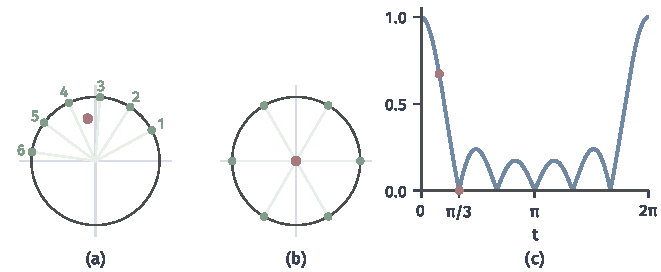
\includegraphics[width=112mm]{figures/07-probability/03-probability-limits/matplotlib/weak-cf-circle/figure.pdf}
 \caption{特征函数是单位圆上的重心。$X$为均匀骰子点数，绿点为$\mathrm{e}^{\mathrm{i}tk}$（$k=1,\dots,6$），每点质量$1/6$，红点为重心$\phi_X(t)$。(a)$t=0.5$；(b)$t=\pi/3$，六点构成正六边形，重心为$0$。(c)$\lvert\phi_X(t)\rvert$，$0\leq t\leq2\pi$，红点对应(a)(b)两个频率。}
 \label{fig:weak-cf-circle}
\end{BookInlineFigure}

\paragraph{基本性质}
由定义直接得到三条性质。第一，$\phi_X(0)=1$，且
\[
 \lvert\phi_X(t)\rvert\leq\mathbb{E}\bigl[\lvert\mathrm{e}^{\mathrm{i}tX}\rvert\bigr]=1 .
\]
第二，共轭对称：$\mathrm{e}^{-\mathrm{i}tX}$是$\mathrm{e}^{\mathrm{i}tX}$的共轭，所以$\phi_X(-t)=\overline{\phi_X(t)}$。若$X$与$-X$同分布，则$\phi_X(t)=\phi_{-X}(t)=\phi_X(-t)$，再由共轭对称，$\phi_X(t)$等于自己的共轭，特征函数是实的。

第三，一致连续。对任意$t$与$h$，
\[
 \lvert\phi_X(t+h)-\phi_X(t)\rvert=\bigl\lvert\mathbb{E}\bigl[\mathrm{e}^{\mathrm{i}tX}(\mathrm{e}^{\mathrm{i}hX}-1)\bigr]\bigr\rvert\leq\mathbb{E}\bigl[\lvert\mathrm{e}^{\mathrm{i}hX}-1\rvert\bigr] .
\]
右边不含$t$。$h\to0$时$\lvert\mathrm{e}^{\mathrm{i}hX}-1\rvert$逐点趋于零且不超过$2$，由支配收敛定理，右边趋于零。随机向量的情形完全相同。

\paragraph{常见分布}
离散分布按定义求和。$X\sim\operatorname{Bern}(p)$时，$\phi_X(t)=1-p+p\,\mathrm{e}^{\mathrm{i}t}$。$N\sim\operatorname{Poisson}(\lambda)$时，用指数函数的幂级数，
\[
 \phi_N(t)=\sum_{k\geq0}\mathrm{e}^{-\lambda}\frac{(\lambda\mathrm{e}^{\mathrm{i}t})^{k}}{k!}=\exp\bigl(\lambda(\mathrm{e}^{\mathrm{i}t}-1)\bigr) .
\]

有密度的分布按定义积分。$X\sim\operatorname{Unif}(-1,1)$时，虚部的被积函数是奇函数，积分为零，
\[
 \phi_X(t)=\frac12\int_{-1}^{1}\cos(tx)\,\mathrm{d}x=\frac{\sin t}{t},\qquad t\neq0 ,
\]
$\phi_X(0)=1$。

标准高斯$Z\sim\mathcal{N}(0,1)$的特征函数用一个微分方程求出。先说明可以在积分号下对$t$求导。对实数$a$，
\[
 \lvert\mathrm{e}^{\mathrm{i}a}-1\rvert=\Bigl\lvert\int_0^a\mathrm{i}\,\mathrm{e}^{\mathrm{i}s}\,\mathrm{d}s\Bigr\rvert\leq\lvert a\rvert .
\]
于是差商满足
\[
 \Bigl\lvert\mathrm{e}^{\mathrm{i}tx}\,\frac{\mathrm{e}^{\mathrm{i}hx}-1}{h}\,\varphi(x)\Bigr\rvert\leq\lvert x\rvert\varphi(x) .
\]
右边可积，由支配收敛定理，
\[
 \phi_Z'(t)=\int_{-\infty}^{\infty}\mathrm{i}x\,\mathrm{e}^{\mathrm{i}tx}\varphi(x)\,\mathrm{d}x .
\]

再用$x\varphi(x)=-\varphi'(x)$分部积分。边界项$\mathrm{e}^{\mathrm{i}tx}\varphi(x)$在$\pm\infty$处为零，于是
\[
 \phi_Z'(t)=-\mathrm{i}\int_{-\infty}^{\infty}\mathrm{e}^{\mathrm{i}tx}\varphi'(x)\,\mathrm{d}x=\mathrm{i}\int_{-\infty}^{\infty}\mathrm{i}t\,\mathrm{e}^{\mathrm{i}tx}\varphi(x)\,\mathrm{d}x=-t\,\phi_Z(t) .
\]
由此$\bigl(\mathrm{e}^{t^2/2}\phi_Z(t)\bigr)'=0$，结合$\phi_Z(0)=1$，得
\begin{equation}
 \phi_Z(t)=\mathrm{e}^{-t^2/2} .
 \label{eq:weak-gaussian-cf}
\end{equation}
标准高斯的特征函数与密度只差一个常数因子，这是后面高斯平滑论证的关键。

\subsection{变换与独立和}
\label{sec:weak-cf-operations}

先看确定的线性变换。对实数$a,b$，把$\mathrm{e}^{\mathrm{i}t(aX+b)}$拆成$\mathrm{e}^{\mathrm{i}tb}$与$\mathrm{e}^{\mathrm{i}(at)X}$之积，取期望得
\begin{equation}
 \phi_{aX+b}(t)=\mathrm{e}^{\mathrm{i}tb}\,\phi_X(at) .
 \label{eq:weak-cf-affine}
\end{equation}
平移只乘一个模为一的因子，不改变$\lvert\phi\rvert$；数乘$a$把频率轴伸缩$a$倍。对随机向量，设$\bm{A}$是$k\times d$矩阵，$\bm{b}\in\mathbb{R}^{k}$。由
\[
 \langle\bm{t},\bm{A}\bm{X}\rangle=\langle\bm{A}^{\top}\bm{t},\bm{X}\rangle ,
\]
得到
\begin{equation}
 \phi_{\bm{A}\bm{X}+\bm{b}}(\bm{t})=\mathrm{e}^{\mathrm{i}\langle\bm{t},\bm{b}\rangle}\,\phi_{\bm{X}}(\bm{A}^{\top}\bm{t}),\qquad\bm{t}\in\mathbb{R}^{k} .
 \label{eq:weak-cf-linear}
\end{equation}

例如$X\sim\mathcal{N}(\mu,\sigma^2)$可以写成$\mu+\sigma Z$，由式~\eqref{eq:weak-gaussian-cf}与式~\eqref{eq:weak-cf-affine}，
\[
 \phi_X(t)=\exp\Bigl(\mathrm{i}\mu t-\frac{\sigma^2t^2}{2}\Bigr) .
\]

\paragraph{独立和}
独立性把乘积的期望拆成期望的乘积，这正是复指数的加法性质需要的。

\begin{theorem}[独立和的特征函数]
\label{thm:weak-cf-independent}
设$\bm{X}$与$\bm{Y}$是相互独立、分别取值于$\mathbb{R}^{d}$与$\mathbb{R}^{k}$的随机向量。则联合特征函数可以分解为
\begin{equation}
 \phi_{(\bm{X},\bm{Y})}(\bm{s},\bm{t})=\phi_{\bm{X}}(\bm{s})\,\phi_{\bm{Y}}(\bm{t}),\qquad\bm{s}\in\mathbb{R}^{d},\ \bm{t}\in\mathbb{R}^{k} .
 \label{eq:weak-cf-joint-independent}
\end{equation}
特别地，$k=d$时，
\begin{equation}
 \phi_{\bm{X}+\bm{Y}}(\bm{t})=\phi_{\bm{X}}(\bm{t})\,\phi_{\bm{Y}}(\bm{t}) .
 \label{eq:weak-cf-sum}
\end{equation}
对相互独立的$\bm{X}_1,\dots,\bm{X}_n$，和的特征函数是$\prod_{j}\phi_{\bm{X}_j}$。
\end{theorem}

\begin{proof}
对有界可测的实函数$g,h$，独立性给出（第~\ref{chap:random-vectors}章）
\[
 \mathbb{E}[g(\bm{X})h(\bm{Y})]=\mathbb{E}[g(\bm{X})]\,\mathbb{E}[h(\bm{Y})] .
\]
把$\mathrm{e}^{\mathrm{i}\langle\bm{s},\bm{X}\rangle}$与$\mathrm{e}^{\mathrm{i}\langle\bm{t},\bm{Y}\rangle}$各自拆成实部与虚部，它们都是有界可测函数，乘开后有四项，每项都按上式分解，再合并，即得式~\eqref{eq:weak-cf-joint-independent}。取$\bm{s}=\bm{t}$，由内积的线性得式~\eqref{eq:weak-cf-sum}。$n$项的情形对$n$归纳。
\end{proof}

用已知分布检验这个公式。$\operatorname{Bin}(n,p)$是$n$个独立$\operatorname{Bern}(p)$之和，按式~\eqref{eq:weak-cf-sum}，
\[
 \phi(t)=\bigl(1-p+p\,\mathrm{e}^{\mathrm{i}t}\bigr)^{n} .
\]
按定义直接求和，由二项式定理，
\[
 \sum_{k=0}^{n}\binom nkp^{k}(1-p)^{n-k}\mathrm{e}^{\mathrm{i}tk}=\bigl(1-p+p\,\mathrm{e}^{\mathrm{i}t}\bigr)^{n} ,
\]
两者一致。独立的$\operatorname{Poisson}(\lambda_1)$与$\operatorname{Poisson}(\lambda_2)$之和，特征函数是$\exp\bigl((\lambda_1+\lambda_2)(\mathrm{e}^{\mathrm{i}t}-1)\bigr)$，正是$\operatorname{Poisson}(\lambda_1+\lambda_2)$的特征函数；下一小节的唯一性定理说明，和就服从这个分布。

多元高斯也可以这样算。设$\bm{Z}=(Z_1,\dots,Z_m)$的分量是独立的标准高斯变量，由式~\eqref{eq:weak-cf-joint-independent}，
\[
 \phi_{\bm{Z}}(\bm{s})=\prod_{j=1}^{m}\mathrm{e}^{-s_j^2/2}=\mathrm{e}^{-\lVert\bm{s}\rVert_2^2/2} .
\]
第~\ref{chap:multivariate-distributions}章把与$\bm{\mu}+\bm{A}\bm{Z}$同分布的随机向量$\bm{X}$定义为服从$\mathcal{N}(\bm{\mu},\bm{\Sigma})$，其中$\bm{\Sigma}=\bm{A}\bm{A}^{\top}$。由式~\eqref{eq:weak-cf-linear}，
\begin{equation}
 \phi_{\bm{X}}(\bm{t})=\exp\Bigl(\mathrm{i}\langle\bm{t},\bm{\mu}\rangle-\frac12\lVert\bm{A}^{\top}\bm{t}\rVert_2^2\Bigr)=\exp\Bigl(\mathrm{i}\langle\bm{t},\bm{\mu}\rangle-\frac12\bm{t}^{\top}\bm{\Sigma}\bm{t}\Bigr) .
 \label{eq:weak-mvn-cf}
\end{equation}
结果只通过$\bm{\Sigma}$依赖$\bm{A}$，与那一章的结论一致；$\bm{\Sigma}$奇异时公式照样成立。

\paragraph{没有独立时}
式~\eqref{eq:weak-cf-sum}离不开独立性。设$X\sim\operatorname{Unif}(-1,1)$，若$Y$是与$X$独立的同分布变量，$X+Y$的密度是$[-2,2]$上的三角形（第~\ref{chap:random-variable-transformations}章的卷积），特征函数是$(\sin t/t)^2$。若取$Y=X$，和是$2X$，由式~\eqref{eq:weak-cf-affine}，特征函数是$\sin(2t)/(2t)$。在$t=\pi/2$处，
\[
 \frac{\sin\pi}{\pi}=0,\qquad\Bigl(\frac{\sin(\pi/2)}{\pi/2}\Bigr)^{2}=\frac{4}{\pi^{2}}\approx0.405 ,
\]
两者不同。图~\ref{fig:weak-cf-sum}把两种和的密度与特征函数并排画出：边缘相同，配对方式不同，和的分布就不同。

\begin{BookInlineFigure}
 \centering
 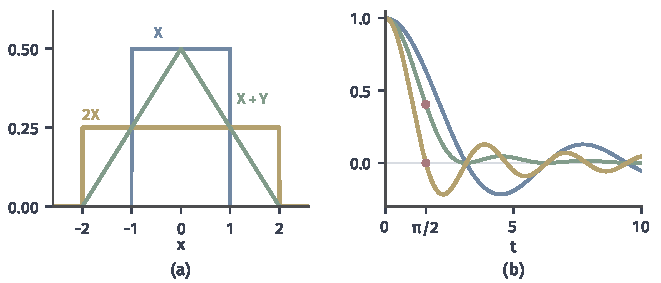
\includegraphics[width=112mm]{figures/07-probability/03-probability-limits/matplotlib/weak-cf-sum/figure.pdf}
 \caption{独立和与非独立和。(a)$\operatorname{Unif}(-1,1)$的密度（蓝），两个独立副本之和的三角形密度（绿），$2X$的均匀密度（黄）。(b)对应的特征函数$\sin t/t$、$(\sin t/t)^2$与$\sin(2t)/(2t)$，红点标出$t=\pi/2$处的两个值$4/\pi^2$与$0$。}
 \label{fig:weak-cf-sum}
\end{BookInlineFigure}

\subsection{矩与局部展开}
\label{sec:weak-cf-moments}

特征函数在原点附近的形状记录了矩。$\mathrm{e}^{\mathrm{i}tx}$对$t$求一次导数多出因子$\mathrm{i}x$，所以对期望求导，若能与期望交换，就得到$\mathbb{E}[\mathrm{i}X\mathrm{e}^{\mathrm{i}tX}]$。交换的条件是相应的绝对矩有限。为了控制余项，先给出复指数Taylor展开的误差界。

\begin{lemma}[复指数的展开误差]
\label{lem:weak-exp-remainder}
对实数$x$与整数$m\geq0$，
\begin{equation}
 \Bigl\lvert\mathrm{e}^{\mathrm{i}x}-\sum_{j=0}^{m}\frac{(\mathrm{i}x)^{j}}{j!}\Bigr\rvert\leq\min\Bigl(\frac{\lvert x\rvert^{m+1}}{(m+1)!},\ \frac{2\lvert x\rvert^{m}}{m!}\Bigr) .
 \label{eq:weak-exp-remainder}
\end{equation}
\end{lemma}

\begin{proof}
记左边绝对值内的量为$R_m(x)$。对$x$求导，
\[
 R_m'(x)=\mathrm{i}\,\mathrm{e}^{\mathrm{i}x}-\sum_{j=1}^{m}\frac{\mathrm{i}(\mathrm{i}x)^{j-1}}{(j-1)!}=\mathrm{i}R_{m-1}(x) ,
\]
又$R_m(0)=0$，所以$R_m(x)=\mathrm{i}\int_0^xR_{m-1}(s)\,\mathrm{d}s$。

对$m$归纳。$m=0$时，$R_0(x)=\mathrm{e}^{\mathrm{i}x}-1$，前面计算高斯特征函数时已经说明它的模不超过$\lvert x\rvert$；又由三角不等式，$\lvert R_0(x)\rvert\leq2$。设结论对$m-1$成立，则
\[
 \lvert R_m(x)\rvert\leq\int_0^{\lvert x\rvert}\min\Bigl(\frac{s^{m}}{m!},\frac{2s^{m-1}}{(m-1)!}\Bigr)\mathrm{d}s .
\]
分别只用最小值中的一项积分，得到$\lvert x\rvert^{m+1}/(m+1)!$与$2\lvert x\rvert^{m}/m!$两个上界。
\end{proof}

两个上界各有用处：$\lvert x\rvert$小时第一个更小，$\lvert x\rvert$大时第二个只增长到$m$次幂。下面的论证会同时用到这两种情形。

\begin{theorem}[矩与导数]
\label{thm:weak-cf-derivatives}
设$k\geq1$为整数，$\mathbb{E}[\lvert X\rvert^{k}]<\infty$。则$\phi_X$有直到$k$阶的连续导数，
\begin{equation}
 \phi_X^{(j)}(t)=\mathbb{E}\bigl[(\mathrm{i}X)^{j}\mathrm{e}^{\mathrm{i}tX}\bigr],\qquad
 \phi_X^{(j)}(0)=\mathrm{i}^{j}\,\mathbb{E}[X^{j}],\qquad j=0,1,\dots,k .
 \label{eq:weak-cf-derivatives}
\end{equation}
\end{theorem}

\begin{proof}
对$j$归纳，$j=0$即定义。设$j<k$时公式成立，考虑差商
\[
 \frac{\phi_X^{(j)}(t+h)-\phi_X^{(j)}(t)}{h}=\mathbb{E}\Bigl[(\mathrm{i}X)^{j}\mathrm{e}^{\mathrm{i}tX}\,\frac{\mathrm{e}^{\mathrm{i}hX}-1}{h}\Bigr] .
\]
由引理~\ref{lem:weak-exp-remainder}（$m=0$），期望内的量的模不超过$\lvert X\rvert^{j+1}$。$j+1\leq k$，且$\lvert X\rvert^{j+1}\leq1+\lvert X\rvert^{k}$，所以它可积。$h\to0$时期望内的量逐点趋于$(\mathrm{i}X)^{j+1}\mathrm{e}^{\mathrm{i}tX}$，由支配收敛定理得到$j+1$阶的公式。导数的连续性同样由支配收敛定理得到，控制函数是$\lvert X\rvert^{j}$。取$t=0$即得原点处的值。
\end{proof}

例如$N\sim\operatorname{Poisson}(2)$，它的特征函数已在第~\ref{sec:weak-cf-definition}节求出。逐次求导，
\[
 \begin{aligned}
 \phi_N'(t)&=2\mathrm{i}\,\mathrm{e}^{\mathrm{i}t}\phi_N(t),\\
 \phi_N''(t)&=\bigl((2\mathrm{i}\,\mathrm{e}^{\mathrm{i}t})^{2}-2\,\mathrm{e}^{\mathrm{i}t}\bigr)\phi_N(t) .
 \end{aligned}
\]
在原点，$\phi_N'(0)=2\mathrm{i}$，$\phi_N''(0)=-4-2=-6$。由式~\eqref{eq:weak-cf-derivatives}，
\[
 \mathbb{E}[N]=2,\qquad\mathbb{E}[N^{2}]=6,\qquad\operatorname{Var}(N)=6-4=2 ,
\]
与第~\ref{chap:common-distributions}章的结果相同。这里先由Poisson分布的各阶矩有限（其尾部比任何幂次都轻）保证求导合法，再读出矩。

\paragraph{二阶展开}
中心极限定理只需要原点附近到二阶的展开，而且只假定二阶矩有限。下面的定理给出展开和余项的控制。

\begin{theorem}[特征函数的二阶展开]
\label{thm:weak-cf-second-order}
设$\mathbb{E}[X^{2}]<\infty$。则
\begin{equation}
 \begin{gathered}
 \phi_X(t)=1+\mathrm{i}t\,\mathbb{E}[X]-\frac{t^{2}}{2}\mathbb{E}[X^{2}]+r(t),\\
 \lvert r(t)\rvert\leq t^{2}\,\mathbb{E}\Bigl[\min\Bigl(\frac{\lvert t\rvert\lvert X\rvert^{3}}{6},\,X^{2}\Bigr)\Bigr] ,
 \end{gathered}
 \label{eq:weak-cf-second-order}
\end{equation}
并且$r(t)/t^{2}\to0$（$t\to0$）。特别地，若$\mathbb{E}[X]=0$，$\operatorname{Var}(X)=\sigma^{2}$，则$\phi_X(t)=1-\sigma^{2}t^{2}/2+r(t)$。
\end{theorem}

\begin{proof}
在引理~\ref{lem:weak-exp-remainder}中取$m=2$，$x=tX$，
\[
 \Bigl\lvert\mathrm{e}^{\mathrm{i}tX}-1-\mathrm{i}tX+\frac{t^{2}X^{2}}{2}\Bigr\rvert\leq\min\Bigl(\frac{\lvert tX\rvert^{3}}{6},\,\lvert tX\rvert^{2}\Bigr)=t^{2}\min\Bigl(\frac{\lvert t\rvert\lvert X\rvert^{3}}{6},\,X^{2}\Bigr) .
\]
取期望，左边期望的模不小于$\lvert r(t)\rvert$，得到式~\eqref{eq:weak-cf-second-order}中的余项界。

$t\to0$时，对每个样本点，余项界中期望内的量不超过$\lvert t\rvert\lvert X\rvert^{3}/6$，因而趋于零；它又被可积的$X^{2}$控制。由支配收敛定理，余项界中的期望趋于零，即$r(t)/t^{2}\to0$。
\end{proof}

这里同时用了引理的两个上界。若只用$\lvert tX\rvert^{3}/6$，就需要三阶矩有限；$X^{2}$这一项让定理只依赖二阶矩，代价是只知道$r(t)=o(t^{2})$，不知道它以什么速度趋于零。

图~\ref{fig:weak-cf-local}比较三个均值为$0$、方差为$1$的分布：以$\pm1$各半取值的变量，特征函数为$\cos t$；$\operatorname{Unif}(-\sqrt3,\sqrt3)$，特征函数为$\sin(\sqrt3t)/(\sqrt3t)$；标准高斯$\mathrm{e}^{-t^{2}/2}$。三条曲线在原点附近都贴着抛物线$1-t^{2}/2$，离开原点后才分开。它们的四阶Taylor系数分别是$1/24$、$3/40$与$1/8$，正是四阶矩除以$4!$的不同。

\begin{BookInlineFigure}
 \centering
 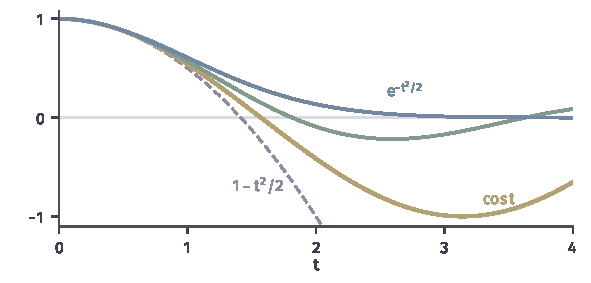
\includegraphics[width=100mm]{figures/07-probability/03-probability-limits/matplotlib/weak-cf-local/figure.pdf}
 \caption{特征函数的二阶展开。均值为$0$、方差为$1$的三个分布：$\pm1$各半（黄，$\cos t$），$\operatorname{Unif}(-\sqrt3,\sqrt3)$（绿），$\mathcal{N}(0,1)$（蓝）；紫色虚线为抛物线$1-t^{2}/2$。}
 \label{fig:weak-cf-local}
\end{BookInlineFigure}

\paragraph{不能反推的部分}
定理~\ref{thm:weak-cf-derivatives}从矩推出导数，反方向只部分成立。若$\phi_X$在原点有二阶导数，可以证明$\mathbb{E}[X^{2}]<\infty$；一般地，原点处存在$2k$阶导数蕴含$2k$阶矩有限。奇数阶则不然：存在对称分布，其特征函数在原点可导，期望$\mathbb{E}[\lvert X\rvert]$却是无穷大，例如尾部$\mathbb{P}(\lvert X\rvert>x)$像$1/(x\ln x)$那样衰减的分布。这些结论的证明可查阅~\scite{math-kallenberg2021probability}。因此，看到特征函数有若干阶导数，不能直接断言对应各阶矩都存在，更不能断言所有矩存在。

\subsection{分布唯一性}
\label{sec:weak-cf-uniqueness}

特征函数要作识别工具，首先必须做到：不同分布的特征函数不同。若分布有可积的密度，这是Fourier变换的单射性；但一般分布可能有原子，也可能既无原子又无密度。办法是先给分布加一点高斯噪声，把它抹成有光滑密度的分布，再让噪声趋于零。

\paragraph{高斯平滑}
平滑要用到高斯密度与其特征函数的对偶。取$\sigma>0$，考虑高斯分布$\mathcal{N}(\bm{0},\sigma^{-2}\bm{I}_d)$，它的密度是
\[
 \Bigl(\frac{\sigma^{2}}{2\pi}\Bigr)^{d/2}\mathrm{e}^{-\sigma^{2}\lVert\bm{s}\rVert_2^{2}/2},\qquad\bm{s}\in\mathbb{R}^{d} .
\]
由式~\eqref{eq:weak-mvn-cf}，它在$\bm{u}$处的特征函数是$\mathrm{e}^{-\lVert\bm{u}\rVert_2^{2}/(2\sigma^{2})}$。把特征函数写成积分，两边乘以常数$(2\pi\sigma^{2})^{-d/2}$，得到
\begin{equation}
 \begin{aligned}
 \frac{1}{(2\pi\sigma^{2})^{d/2}}\mathrm{e}^{-\lVert\bm{u}\rVert_2^{2}/(2\sigma^{2})}
 &=\frac{1}{(2\pi)^{d}}\int_{\mathbb{R}^{d}}\mathrm{e}^{\mathrm{i}\langle\bm{s},\bm{u}\rangle}\mathrm{e}^{-\sigma^{2}\lVert\bm{s}\rVert_2^{2}/2}\,\mathrm{d}\bm{s} .
 \end{aligned}
 \label{eq:weak-gauss-identity}
\end{equation}
左边是$\mathcal{N}(\bm{0},\sigma^{2}\bm{I}_d)$的密度，记作$g_{\sigma}(\bm{u})$。式~\eqref{eq:weak-gauss-identity}把它写成了复指数的叠加。

设$\bm{Z}\sim\mathcal{N}(\bm{0},\bm{I}_d)$与$\bm{X}$独立（必要时在乘积空间上构造）。给定$\bm{X}=\bm{x}_0$，$\bm{X}+\sigma\bm{Z}$服从以$\bm{x}_0$为中心的$\mathcal{N}(\bm{x}_0,\sigma^{2}\bm{I}_d)$。由独立性与Tonelli定理，对每个Borel集$A$，
\[
 \mathbb{P}(\bm{X}+\sigma\bm{Z}\in A)=\mathbb{E}\Bigl[\int_Ag_{\sigma}(\bm{x}-\bm{X})\,\mathrm{d}\bm{x}\Bigr]=\int_A\mathbb{E}\bigl[g_{\sigma}(\bm{x}-\bm{X})\bigr]\,\mathrm{d}\bm{x} .
\]
所以$\bm{X}+\sigma\bm{Z}$有密度
\[
 f_{\sigma}(\bm{x})=\mathbb{E}\bigl[g_{\sigma}(\bm{x}-\bm{X})\bigr] ,
\]
这就是把$\bm{X}$的每一份质量用一个小高斯“抹开”后的结果。

把式~\eqref{eq:weak-gauss-identity}代入$f_{\sigma}$，并交换期望与积分。被积函数的模不超过$\mathrm{e}^{-\sigma^{2}\lVert\bm{s}\rVert_2^{2}/2}$，它在乘积空间上可积，Fubini定理适用。于是
\begin{equation}
 f_{\sigma}(\bm{x})=\frac{1}{(2\pi)^{d}}\int_{\mathbb{R}^{d}}\mathrm{e}^{\mathrm{i}\langle\bm{s},\bm{x}\rangle}\,\phi_{\bm{X}}(-\bm{s})\,\mathrm{e}^{-\sigma^{2}\lVert\bm{s}\rVert_2^{2}/2}\,\mathrm{d}\bm{s} .
 \label{eq:weak-smoothed-density}
\end{equation}
平滑后的密度完全由特征函数算出。

\begin{theorem}[特征函数确定分布]
\label{thm:weak-cf-uniqueness}
设$\bm{X}$与$\bm{Y}$是取值于$\mathbb{R}^{d}$的随机向量。若$\phi_{\bm{X}}(\bm{t})=\phi_{\bm{Y}}(\bm{t})$对一切$\bm{t}\in\mathbb{R}^{d}$成立，则$P_{\bm{X}}=P_{\bm{Y}}$。
\end{theorem}

\begin{proof}
取$\bm{Z}$与$\bm{X}$独立，$\bm{Z}'$与$\bm{Y}$独立，都服从$\mathcal{N}(\bm{0},\bm{I}_d)$。由式~\eqref{eq:weak-smoothed-density}，对每个$\sigma>0$，$\bm{X}+\sigma\bm{Z}$与$\bm{Y}+\sigma\bm{Z}'$的密度相同，因而分布相同。

取$\sigma=1/m$。对每个样本点，$\bm{X}+\bm{Z}/m\to\bm{X}$，所以依概率收敛，由定理~\ref{thm:weak-prob-implies-dist}也依分布收敛；同样$\bm{Y}+\bm{Z}'/m\xrightarrow{\mathrm{d}}\bm{Y}$。两列随机向量的分布逐项相同，是同一个分布列，它同时弱收敛到$P_{\bm{X}}$与$P_{\bm{Y}}$。由引理~\ref{lem:weak-uniqueness}，$P_{\bm{X}}=P_{\bm{Y}}$。
\end{proof}

证明只用了弱收敛的定义、依概率收敛与依分布收敛的关系，以及极限唯一性，没有用到联合分布的极限判据。图~\ref{fig:weak-gaussian-smoothing}显示了平滑与还原：$\operatorname{Poisson}(2)$只有原子，没有密度；式~\eqref{eq:weak-smoothed-density}算出的$f_\sigma$在每个原子处鼓起一个小包，$\sigma$越小，小包越窄越高，质量越来越集中到原子上。

\begin{BookInlineFigure}
 \centering
 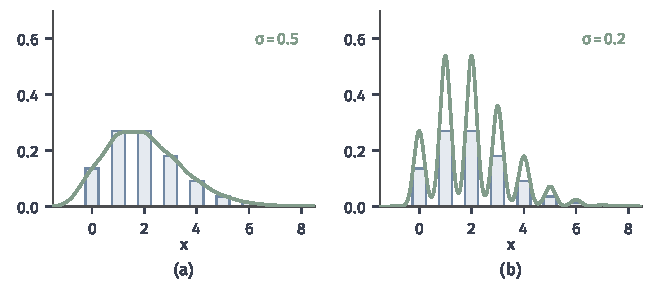
\includegraphics[width=112mm]{figures/07-probability/03-probability-limits/matplotlib/weak-gaussian-smoothing/figure.pdf}
 \caption{高斯平滑。浅蓝柱为$\operatorname{Poisson}(2)$在$k=0,\dots,7$的质量。曲线是由式~\eqref{eq:weak-smoothed-density}对特征函数数值积分得到的平滑密度$f_\sigma$：(a)$\sigma=0.5$（绿）；(b)$\sigma=0.2$（绿）。脚本同时按“各原子处放一个高斯小包”直接计算并核对两种结果相同。}
 \label{fig:weak-gaussian-smoothing}
\end{BookInlineFigure}

\paragraph{反演公式}
若$\phi_{\bm{X}}$本身在$\mathbb{R}^{d}$上可积，可以在式~\eqref{eq:weak-smoothed-density}中直接令$\sigma\to0$：被积函数被可积的$\lvert\phi_{\bm{X}}\rvert$控制，由支配收敛定理，$f_\sigma$一致收敛到
\begin{equation}
 f(\bm{x})=\frac{1}{(2\pi)^{d}}\int_{\mathbb{R}^{d}}\mathrm{e}^{-\mathrm{i}\langle\bm{t},\bm{x}\rangle}\,\phi_{\bm{X}}(\bm{t})\,\mathrm{d}\bm{t}
 \label{eq:weak-inversion}
\end{equation}
（积分变量换成了$\bm{t}=-\bm{s}$），这就是\term{反演公式}（inversion formula）。对连续且支撑有界的函数$h$，一方面$\mathbb{E}[h(\bm{X}+\sigma\bm{Z})]$等于$\int hf_\sigma$，趋于$\int hf$；另一方面由定理~\ref{thm:weak-prob-implies-dist}，它趋于$\mathbb{E}[h(\bm{X})]$。用这样的$h$从上方逼近闭长方体的示性函数，与引理~\ref{lem:weak-uniqueness}同样的单调极限说明，$\bm{X}$有连续密度$f$。这与\BookChapterRef{chap:fourier-transform}{卷四第14章“Fourier变换”}的$L^{1}$反演定理是同一件事，那里的约定在指数中带有$2\pi$，常数因而不同。

用反演公式可以求出一个不易直接积分的特征函数。$\operatorname{Laplace}(0,1)$的密度为$\frac12\mathrm{e}^{-\lvert x\rvert}$，它对称，特征函数为
\[
 \int_0^{\infty}\mathrm{e}^{-x}\cos(tx)\,\mathrm{d}x=\frac{1}{1+t^{2}} .
\]
它可积，由式~\eqref{eq:weak-inversion}，
\[
 \frac12\mathrm{e}^{-\lvert x\rvert}=\frac{1}{2\pi}\int_{-\infty}^{\infty}\frac{\mathrm{e}^{-\mathrm{i}tx}}{1+t^{2}}\,\mathrm{d}t .
\]
交换$x$与$t$的名字，两边乘以$2$。右边的被积函数中，Cauchy密度对称，$\mathrm{e}^{-\mathrm{i}tx}$可以换成$\mathrm{e}^{\mathrm{i}tx}$，于是右边就是标准Cauchy分布（密度$1/(\pi(1+x^{2}))$）在$t$处的特征函数，它等于$\mathrm{e}^{-\lvert t\rvert}$。

Cauchy分布的特征函数在原点不可导，与它没有期望相符。它还说明式~\eqref{eq:weak-cf-sum}的逆命题不成立：设$X$服从标准Cauchy分布，取$Y=X$，则
\[
 \phi_{X+Y}(t)=\phi_X(2t)=\mathrm{e}^{-2\lvert t\rvert}=\phi_X(t)\,\phi_Y(t) ,
\]
乘积公式成立，而$X$与$Y$并不独立。

\paragraph{有界变量的矩}
第~\ref{chap:random-variable-moments}章提到，取值有界时全部矩决定分布。现在可以证明这一点。设$\lvert X\rvert\leq M$，在引理~\ref{lem:weak-exp-remainder}中取$x=tX$并取期望，
\[
 \Bigl\lvert\phi_X(t)-\sum_{j=0}^{m}\frac{(\mathrm{i}t)^{j}}{j!}\mathbb{E}[X^{j}]\Bigr\rvert\leq\frac{(\lvert t\rvert M)^{m+1}}{(m+1)!}\longrightarrow0\qquad(m\to\infty) .
\]
所以对每个$t$，
\[
 \phi_X(t)=\sum_{j\geq0}\frac{(\mathrm{i}t)^{j}}{j!}\mathbb{E}[X^{j}] .
\]
两个有界变量若各阶矩相同，特征函数就相同，由定理~\ref{thm:weak-cf-uniqueness}，分布也相同。第~\ref{sec:weak-mgf}节将把有界的条件放宽为指数矩有限，并看到不加条件时结论可能失败。

\subsection{连续性定理}
\label{sec:weak-cf-continuity}

现在回到弱收敛。$\cos\langle\bm{t},\bm{x}\rangle$与$\sin\langle\bm{t},\bm{x}\rangle$是有界连续函数，所以弱收敛时特征函数逐点收敛。反过来，若特征函数逐点收敛，分布是否弱收敛？还要排除质量逃逸。

先看反例。$X_n\sim\mathcal{N}(0,n)$的特征函数是$\mathrm{e}^{-nt^{2}/2}$，它在$t=0$处恒为$1$，在$t\neq0$处趋于$0$。逐点极限
\[
 \psi(t)=\begin{cases}1,&t=0,\\0,&t\neq0\end{cases}
\]
存在，但在原点不连续；而第~\ref{sec:weak-tightness}节已经看到，这列分布的质量逃向无穷远，没有弱极限。原点附近的特征函数对应低频，也就是大尺度的形状；质量跑远，正表现为低频部分的塌缩。下面的引理把这个直观写成不等式。

\begin{lemma}[由特征函数控制尾概率]
\label{lem:weak-cf-tail}
设$X$是实随机变量，$u>0$，则
\begin{equation}
 \mathbb{P}\bigl(\lvert X\rvert\geq2/u\bigr)\leq\frac1u\int_{-u}^{u}\bigl(1-\phi_X(t)\bigr)\,\mathrm{d}t .
 \label{eq:weak-cf-tail}
\end{equation}
右边是实数，因为$\phi_X$的虚部是奇函数，积分为零。
\end{lemma}

\begin{proof}
对固定的$x\neq0$，
\[
 \frac1u\int_{-u}^{u}\bigl(1-\mathrm{e}^{\mathrm{i}tx}\bigr)\,\mathrm{d}t=2-\frac{2\sin(ux)}{ux}=2\Bigl(1-\frac{\sin(ux)}{ux}\Bigr) ,
\]
$x=0$时左边为$0$。被积函数有界，由Fubini定理交换期望与积分，
\[
 \frac1u\int_{-u}^{u}\bigl(1-\phi_X(t)\bigr)\,\mathrm{d}t=2\,\mathbb{E}\Bigl[1-\frac{\sin(uX)}{uX}\Bigr] ,
\]
其中$uX=0$时方括号内取$0$。

对一切实数$y\neq0$有$\lvert\sin y/y\rvert\leq1$，所以$1-\sin y/y\geq0$；当$\lvert y\rvert\geq2$时$\lvert\sin y/y\rvert\leq1/\lvert y\rvert\leq1/2$，所以$1-\sin y/y\geq1/2$。于是
\[
 2\,\mathbb{E}\Bigl[1-\frac{\sin(uX)}{uX}\Bigr]\geq2\cdot\frac12\,\mathbb{P}\bigl(\lvert uX\rvert\geq2\bigr)=\mathbb{P}\bigl(\lvert X\rvert\geq2/u\bigr) .
\]
\end{proof}

\begin{theorem}[连续性定理]
\label{thm:weak-continuity}
设$P_n$是$\mathbb{R}^{d}$上的概率分布，特征函数为$\phi_n$。
\begin{enumerate}
 \item 若$P_n\xrightarrow{\mathrm{w}}P$，则$\phi_n(\bm{t})\to\phi_P(\bm{t})$对每个$\bm{t}$成立。
 \item 若$\phi_n(\bm{t})$对每个$\bm{t}$收敛到某个$\psi(\bm{t})$，并且$\psi$在$\bm{0}$处连续，则存在概率分布$P$，使$\psi=\phi_P$且$P_n\xrightarrow{\mathrm{w}}P$。
\end{enumerate}
\end{theorem}

\begin{proof}
(1)：对固定的$\bm{t}$，$\phi_n(\bm{t})$的实部与虚部是有界连续函数$\cos\langle\bm{t},\bm{x}\rangle$与$\sin\langle\bm{t},\bm{x}\rangle$的读数，由定义~\ref{def:weak-convergence}收敛。

(2)：分两步。第一步证明$\{P_n\}$胎紧，先看$d=1$。$\psi(0)=\lim\phi_n(0)=1$。任取$\varepsilon>0$，由$\psi$在原点连续，取$u>0$使$\lvert1-\psi(t)\rvert\leq\varepsilon/2$对$\lvert t\rvert\leq u$成立，于是
\[
 \Bigl\lvert\frac1u\int_{-u}^{u}\bigl(1-\psi(t)\bigr)\,\mathrm{d}t\Bigr\rvert\leq\varepsilon .
\]
$\lvert1-\phi_n\rvert\leq2$，由支配收敛定理，
\[
 \frac1u\int_{-u}^{u}\bigl(1-\phi_n(t)\bigr)\,\mathrm{d}t\longrightarrow\frac1u\int_{-u}^{u}\bigl(1-\psi(t)\bigr)\,\mathrm{d}t .
\]
所以存在$N$，当$n\geq N$时左边小于$2\varepsilon$，由引理~\ref{lem:weak-cf-tail}，
\[
 P_n\bigl(\lvert x\rvert\geq2/u\bigr)<2\varepsilon,\qquad n\geq N .
\]
前$N-1$个分布各自胎紧，与之合并，整列胎紧。

$d>1$时，第$j$个坐标$x_j=\langle\bm{e}_j,\bm{x}\rangle$在$P_n$下的特征函数是$s\mapsto\phi_n(s\bm{e}_j)$，它逐点趋于$s\mapsto\psi(s\bm{e}_j)$，后者在$0$处连续。由一维的结论，每个坐标的分布胎紧。再由
\[
 P_n\bigl(\lVert\bm{x}\rVert_2>r\bigr)\leq\sum_{j=1}^{d}P_n\bigl(\lvert x_j\rvert>r/\sqrt{d}\bigr) ,
\]
$\{P_n\}$胎紧。

第二步识别极限。由定理~\ref{thm:weak-prokhorov}，$\{P_n\}$的每个子列都有进一步的子列弱收敛。设某个子列$P_{n_k}\xrightarrow{\mathrm{w}}Q$，由(1)，$\phi_Q=\lim\phi_{n_k}=\psi$。所以每个子列极限的特征函数都是$\psi$，由定理~\ref{thm:weak-cf-uniqueness}，它们是同一个分布，记作$P$。由引理~\ref{lem:weak-subsequence}，$P_n\xrightarrow{\mathrm{w}}P$，并且$\phi_P=\psi$。
\end{proof}

定理~\ref{thm:weak-continuity}常称为\term{Lévy连续性定理}（Lévy continuity theorem）。(2)的两步对应第~\ref{sec:weak-tightness}节末尾所说的两件事。原点连续性只用在第一步：它通过引理~\ref{lem:weak-cf-tail}保证质量不逃逸。识别极限则交给唯一性定理。结论中$\psi$是特征函数这一点也是证明的产物，并不需要事先知道。

\paragraph{再看二项分布到Poisson分布}
用连续性定理可以不经质量表重新证明$\operatorname{Bin}(n,2/n)\xrightarrow{\mathrm{w}}\operatorname{Poisson}(2)$。需要一个比较乘积的引理，它在下一章的中心极限定理中也要用到。

\begin{lemma}[乘积之差]
\label{lem:weak-product-difference}
设复数$a_1,\dots,a_n$与$b_1,\dots,b_n$的模都不超过$1$，则
\begin{equation}
 \Bigl\lvert\prod_{j=1}^{n}a_j-\prod_{j=1}^{n}b_j\Bigr\rvert\leq\sum_{j=1}^{n}\lvert a_j-b_j\rvert .
 \label{eq:weak-product-difference}
\end{equation}
\end{lemma}

\begin{proof}
$n=1$时是等式。设$n-1$时成立，把差拆成两部分：
\[
 \prod_{j=1}^{n}a_j-\prod_{j=1}^{n}b_j=a_n\Bigl(\prod_{j<n}a_j-\prod_{j<n}b_j\Bigr)+(a_n-b_n)\prod_{j<n}b_j .
\]
$\lvert a_n\rvert\leq1$，$\lvert\prod_{j<n}b_j\rvert\leq1$，由三角不等式与归纳假设即得。
\end{proof}

设$X_n\sim\operatorname{Bin}(n,2/n)$，记$z=2(\mathrm{e}^{\mathrm{i}t}-1)$，则
\[
 \phi_{X_n}(t)=\Bigl(1+\frac zn\Bigr)^{n},\qquad\exp\bigl(2(\mathrm{e}^{\mathrm{i}t}-1)\bigr)=\bigl(\mathrm{e}^{z/n}\bigr)^{n} .
\]
$n\geq2$时，$1+z/n=(1-2/n)+(2/n)\mathrm{e}^{\mathrm{i}t}$是单位圆盘中两点的凸组合，模不超过$1$；$z$的实部$2(\cos t-1)\leq0$，所以$\lvert\mathrm{e}^{z/n}\rvert\leq1$。

由引理~\ref{lem:weak-product-difference}，
\[
 \bigl\lvert\phi_{X_n}(t)-\mathrm{e}^{z}\bigr\rvert\leq n\,\Bigl\lvert1+\frac zn-\mathrm{e}^{z/n}\Bigr\rvert .
\]
对$\lvert w\rvert\leq1$，由幂级数，
\[
 \lvert\mathrm{e}^{w}-1-w\rvert\leq\sum_{k\geq2}\frac{\lvert w\rvert^{k}}{k!}\leq\lvert w\rvert^{2}(\mathrm{e}-2)\leq\lvert w\rvert^{2} .
\]
$\lvert z\rvert\leq4$，取$n\geq4$与$w=z/n$，得到
\[
 \bigl\lvert\phi_{X_n}(t)-\exp\bigl(2(\mathrm{e}^{\mathrm{i}t}-1)\bigr)\bigr\rvert\leq n\cdot\frac{\lvert z\rvert^{2}}{n^{2}}\leq\frac{16}{n} .
\]
所以特征函数收敛到$\operatorname{Poisson}(2)$的特征函数，后者连续，由连续性定理即得弱收敛。

以$t=\pi$为例，$z=-4$，$\phi_{X_n}(\pi)=(1-4/n)^{n}$。$n=10$与$n=40$时依次为
\[
 0.6^{10}\approx0.00605,\qquad0.9^{40}\approx0.0148 ,
\]
极限为$\mathrm{e}^{-4}\approx0.0183$。图~\ref{fig:weak-continuity}(a)画出特征函数实部的收敛；(b)是$\mathcal{N}(0,n)$的反例，极限在原点断开。

\begin{BookInlineFigure}
 \centering
 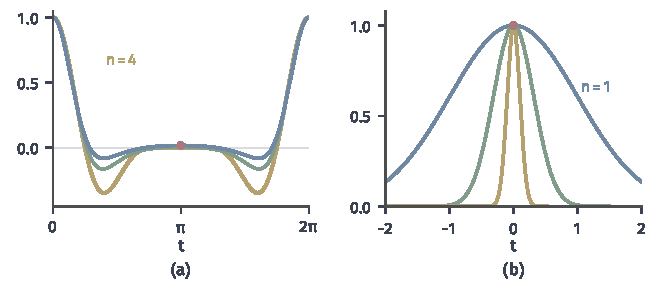
\includegraphics[width=112mm]{figures/07-probability/03-probability-limits/matplotlib/weak-continuity/figure.pdf}
 \caption{连续性定理的两种情形。(a)$\operatorname{Bin}(n,2/n)$特征函数的实部，$n=4$（黄）、$10$（绿），蓝线为$\operatorname{Poisson}(2)$的$\operatorname{Re}\exp(2(\mathrm{e}^{\mathrm{i}t}-1))$，红点为$t=\pi$处的极限$\mathrm{e}^{-4}$。(b)$\mathcal{N}(0,n)$的特征函数$\mathrm{e}^{-nt^2/2}$，$n=1$（蓝）、$10$（绿）、$100$（黄），逐点极限在原点为$1$（红点）、其余为$0$。}
 \label{fig:weak-continuity}
\end{BookInlineFigure}
